
\subsection{Analyse Vodafone}
Vodafone hat nur wenig Kriterien verletzt. Genauer gesagt zwei. Dagegen sind pro Kriterium eine große Anzahl an Fehlern aufgetreten.

Der mit Abstand häufigste Fehler ist der Verstoß gegen Kriterium 1.1.1 \enquote{Nicht-Text-Inhalt}. Dabei sind nicht nur Bilder betroffen.

\begin{figure}[H]
    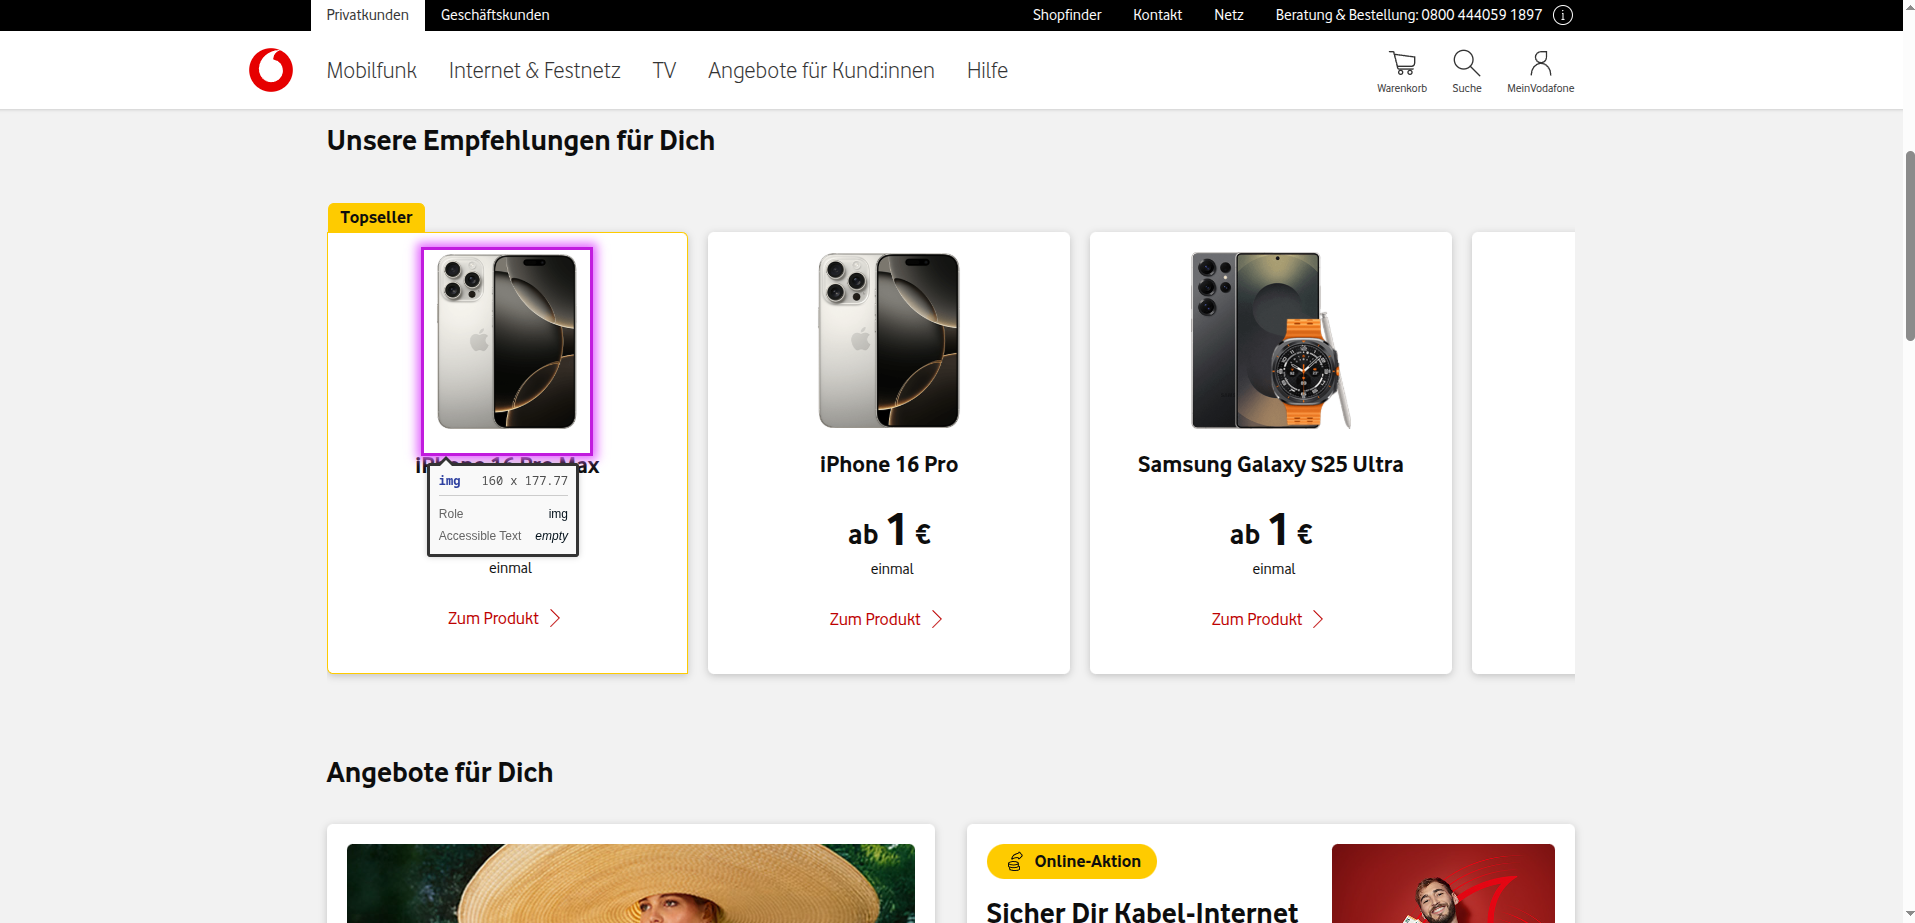
\includegraphics[width=\textwidth]{img/vodafone_no-alt-text.png}
    \caption{Fehlender alternativer Text bei einem Bild}
\end{figure}

Auch Icons wie in Abbildung 4.28 haben keinen alternativen Text. In diesem Fall handelt es sich um den Button, mit dem man den Slider weiter bewegen kann. Das ist für die Tastaturbedienbarkeit kein wichtiger Button, da man sowieso durch die Elemente hindurch navigieren kann. Aber für Screenreader ist es wichtig, dass der Button auch einen alternativen Text hat, sonst ist es ein Element, das nicht mehr zu erkennen ist.
\begin{figure}[H]
    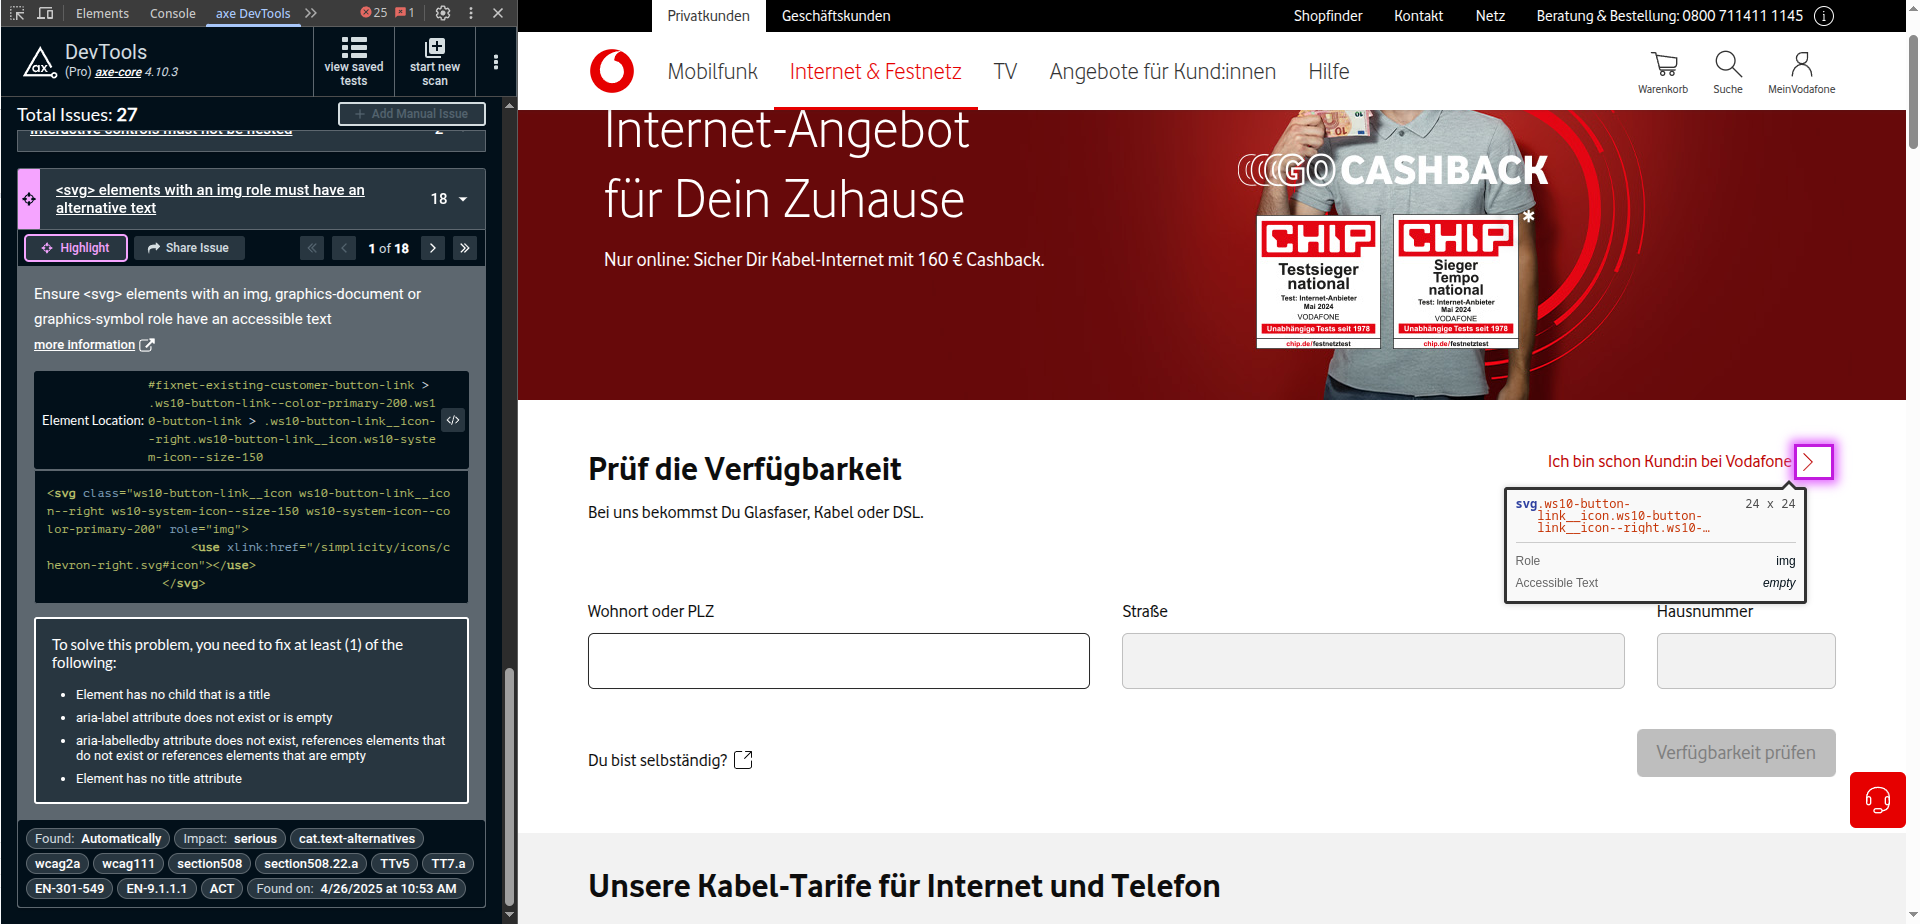
\includegraphics[width=\textwidth]{img/vodafone_no-accessible-text.png}
    \caption{Fehlender alternativer Text beim Slider-Button}
\end{figure}

In der Gesamtbetrachtung der Analyse fällt auf, dass es nur zwei verletzte Kriterien, aber dort dann viele Fehler gibt. Das Kriterium 1.1.1 \enquote{Nicht-textueller Inhalt} ist mit Abstand am häufigsten betroffen. Das zweite Kriterium ist 4.1.2 \enquote{Name, Rolle, Wert}. Hier geht es um die korrekte Benennung der Elemente.

\begin{figure}[H]
\begin{tikzpicture}
\begin{axis}[
    width=\textwidth,
    height=10cm,
    ybar,
    bar width=12pt,
    xlabel={WCAG-Kriterium},
    ylabel={Fehleranzahl},
    symbolic x coords={ 9.1.1.1, 9.4.1.2 },
    xtick=data,
    x tick label style={rotate=45, anchor=east},
    ymin=0,
    ymax=300,
    enlarge x limits=0.1,
    legend style={cells={anchor=west}, legend pos=north east},
    nodes near coords,
    nodes near coords style={font=\scriptsize},
]
\addplot table[x=WCAG-Kriterium,y=Fehleranzahl_axe,col sep=tab] {csv/output/wcag_analyse_Vodafone_xxxx.csv};
\addplot table[x=WCAG-Kriterium,y=Fehleranzahl_WAVE,col sep=tab] {csv/output/wcag_analyse_Vodafone_xxxx.csv};
\legend{axe,WAVE}
\end{axis}
\end{tikzpicture}
\caption{Auswertung Analyse Vodafone}
\end{figure}
